\chapterimage{cover_6.jpg} % Chapter heading image
\chapter{Limitations and Classfication}

This chapter includes the work done to detect static gestures. It begins by describing the general idea of segmentation and recognition and then proceeds to the following sections.\bigskip

\section{Assumptions and Limitations}\index{Assumptions and Limitations}
Every recognition algorithm requires the surrounding environment to assist the process. Our recognition techniques require some assumptions about the surroundings of the process in order to perform its functionality. These assumptions are as follow:\bigskip

\begin{enumerate}

\item No Skin color exits elsewhere in the captured frame. Otherwise, this will affect the color segmentation changes and many other stage such extracting the blob area and perimeter.

\item The Hand is the largest connected component in the image frame. This is based on the nature of the device we developed our work to work on, the glass. The hand before the glass is always the largest object in the frame.
\bigskip

\item The balm of the hand must be separated from the arm by some black cover or anything colored differently from the hand at its rest. 
\bigskip

\item The closed hand is a special static gesture responsible for separating between the recognition of a gesture and the next one. 
\bigskip

\item The dynamic gestures are restricted to just the basic directions; up, down, left, and right. This assumption has its advantages concerning the processing time and the overhead over any application. Yet the interpretation of the four directions is depending essentially on the application. 
\bigskip

\item The separator introduced in the 4th assumption is not applied on dynamic gestures. Dynamic gestures as will be seen are computed between every two frames of motion. As long as the hand is moving, the change in the motion's direction is detected. However, the transition between static gestures and dynamic gestures and vice versa requires the separator to be detected first. 
\end{enumerate}
\bigskip

The algorithms we are about to introduce work at acceptable accuracy in the presence of these assumptions. Otherwise, some performance degradation can fatally harm the results of the algorithm. As it is referenced in the future work chapter, overcoming these challenges and limitations is considered to be an optimization for the functionalities of our algorithm and we encourage everyone interested to provide solutions. 
\bigskip


\section{Classification} \index{Classification}
Our Dataset of gestures contains exactly 234 images. These images are different views for our 8 gestures. Every view is represented as a 1-D Array. The group of images or views is acting as a reference for the classifier to check every query image against it. For every gesture there is a label that the classifier, when its job is done, decides, according to this classifier's algorithm, to which label the query image belongs. The following is our gestures and with how many views they are represented in the dataset:

\paragraph{Start Gesture}\index{Start Gesture}
The gesture is represented by the Ok sign (3 fingers) as shown in Figure \ref{fig:set1} (a). This gesture is marking the start of the detection for any gesture to come forth. It is represented with 18 views in the dataset.

\paragraph{Open Hand}\index{Open Hand}
This gesture is represented by the full hand opened and exposed to the camera as show in Figure \ref{fig:set1} (b). This gesture can be interpreted in many ways according to the application. For example, stop and play in music player. In the dataset, this gesture is represented by 22 views including left and right hands.

\paragraph{Closed Hand}\index{Closed Hand}
This gesture is represented by the full hand closed, fist, and exposed to the camera as show in Figure \ref{fig:set1}(c). This gesture has a special rule. It acts as a separator between the gestures detection i.e. if we detected a gesture, we cannot hope to detect one another following it until the algorithm, any of them receives the fist gesture. In the dataset, this gesture is represented by 14 views.

\paragraph{Capture Gesture}\index{Capture Gesture}
This gesture is represented by a hand shaping a letter C as show in Figure \ref{fig:set1}(d). This gesture has a specific need which is to signal the camera to be opened for capturing an image and capturing after the camera is running. In the dataset, this gesture is represented by 54 view including left and right hands. 

\begin{figure*}[h]
\begin{dBox}
\centering
  \mbox{
      \subfigure[Start Gesture]{
            \label{fig:ok}
            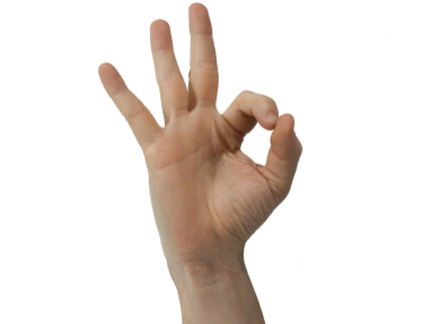
\includegraphics[width=.31\textwidth]{./Pictures/gesture/ok.jpg}
        }
        \subfigure[Open Hand Gesture]{
           \label{fig:open_g}
           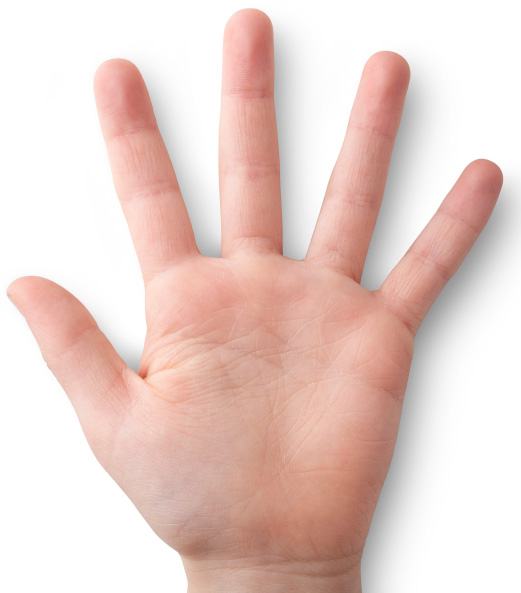
\includegraphics[width=.25\textwidth]{./Pictures/gesture/open.jpg}
        }
        \subfigure[Closed Hand Gesture]{
            \label{fig:closed_g}
            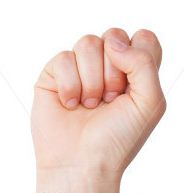
\includegraphics[width=.28\textwidth]{./Pictures/gesture/closed.jpg}
       }
        \subfigure[Capture Gesture]{
            \label{fig:capture_g}
            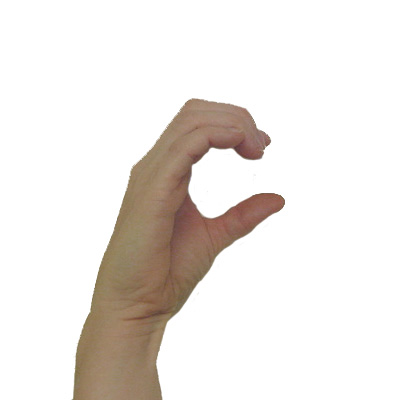
\includegraphics[width=.31\textwidth]{./Pictures/gesture/capture.jpg}
       }
   }
   \caption{Defined Gestures Set 1 \label{fig:set1} }   
\end{dBox}   
\end{figure*}

\paragraph{Call Gesture}\index{Classification}
This gesture is represented by the thumb and the little finger and exposed to the camera as show in Figure \ref{fig:set2}(a). This gesture is used specifically to open the dialer or actually signal to call a number. In the dataset, this gesture is represented by 31 view including left and right hands.

\paragraph{Up Gesture}\index{Classification}
This gesture is represented index finger pointing up and exposed to the camera as show in Figure \ref{fig:set2}(b). This gesture has a special role in our set. It marks the start of detecting a dynamic gesture as mentioned in the dynamic gesture chapter. In the dataset, this gesture is represented by 24 view including left and right hands. 

\paragraph{Right Gesture}\index{Classification}
This gesture is represented by the thumb pointing to the right and exposed to the camera as show in Figure \ref{fig:set2}(c). This gesture can be interpreted in many ways according to the application. For example, stop and play in music player. In the dataset, this gesture is represented by 30 views. 

\paragraph{Left Gesture}\index{Classification}
This gesture is represented by the thumb pointing to the left and exposed to the camera as show in Figure \ref{fig:set2}(d). This gesture can be interpreted in many ways according to the application. For example, stop and play in music player. In the dataset, this gesture is represented by 22 views.

\begin{figure*}[h]
\begin{dBox}
\centering
  \mbox{
      \subfigure[Call Gesture]{
            \label{fig:call}
            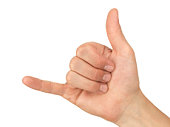
\includegraphics[width=.31\textwidth]{./Pictures/gesture/call.jpg}
        }
        \subfigure[Up Gesture]{
           \label{fig:up_g}
           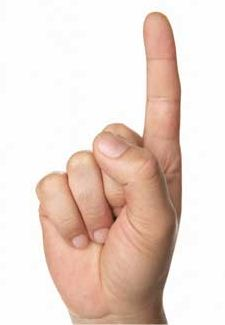
\includegraphics[width=.23\textwidth]{./Pictures/gesture/up.jpg}
        }
        \subfigure[Right Gesture]{
            \label{fig:right_g}
            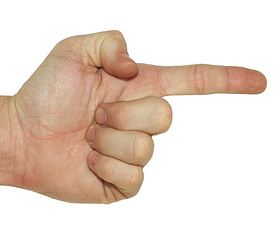
\includegraphics[width=.31\textwidth]{./Pictures/gesture/right.jpg}
       }
        \subfigure[Left Gesture]{
            \label{fig:left_g}
            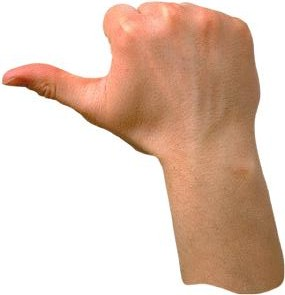
\includegraphics[width=.23\textwidth]{./Pictures/gesture/left.jpg}
       }
   }
   \caption{Defined Gestures Set 2 \label{fig:set2} }   
\end{dBox}   
\end{figure*}

Every algorithm from the previous chapter passes a 1-D array to the classifier. This 1-D array is the classifier input. In the following sections, we are going to represent the three classifiers we used, for our work and how they use this 1-D array. \bigskip

\subsection{Support Vector Machine}\index{Support Vector Machine}
SVM method for the classification of both linear and nonlinear data \cite{classifications}. The algorithm works as follows. It uses a nonlinear mapping to transform the original training data into a higher dimension. Within this new dimension, it searches for the linear optimal separating hyperplane (i.e., a "decision boundary" separating the tuples of one class from another). With an appropriate nonlinear mapping to a sufficiently high dimension, data from two classes can always be separated by a hyperplane. The SVM finds this hyperplane using support vectors ("essential" training tuples) and margins (defined by the support vectors).We will delve more into these new concepts later.


Although the training time of even the fastest SVMs can be extremely slow, they are highly accurate, owing to their ability to model complex nonlinear decision boundaries. They are much less prone to overfitting than other methods. The support vectors found also provide a compact description of the learned model. SVMs can be used for numeric prediction as well as classification. They have been applied to a number of areas, including handwritten digit recognition, object recognition, and speaker identification, as well as benchmark time-series prediction tests.
 \bigskip
\subsubsection{Linear Separability Of The Data}
To explain the mystery of SVMs, let's first look at the simplest case; a two-class problem where the classes are linearly separable. Let the data set D be given as (X1, y1),
(X2, y2), ... , (XD, yD), where Xi is the set of training tuples with associated class labels, yi. Each yi can take one of two values, either +1 or -1 (i.e., $yi \subseteq{+1,-1}$), corresponding to the classes buys computer D yes and buys computer D no, respectively.\bigskip

To aid in visualization, let's consider an example based on two input attributes, A1 and A2, as shown in Figure \ref{fig:svm1}. From the graph, we see that the 2-D data are linearly separable (or "linear" for short), because a straight line can be drawn to separate all the tuples of class +1 from all the tuples of class -1.\bigskip

\begin{figure*}[h]
\begin{dBox}
\centering
  \mbox{
      \subfigure[]{
            \label{fig:svm_1}
            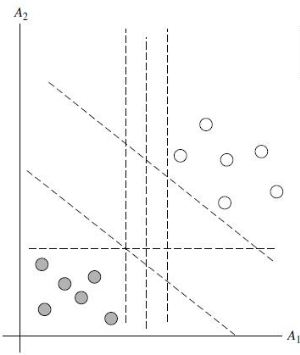
\includegraphics[width=.31\textwidth]{./Pictures/gesture/svm1.jpg}
        }
   }
   \caption{SVM Separability Idea \cite{classifications}\label{fig:svm1} }   
\end{dBox}   
\end{figure*}

There are an infinite number of separating lines that could be drawn. We want to find the "best" one, that is, one that will have the minimum classification error on previously unseen tuples. How can we find this best line? Note that if our data were 3-D (i.e., with three attributes); we would want to find the best separating plane. Generalizing to n dimensions, we want to find the best hyperplane. We will use "hyperplane" to refer to the decision boundary that we are seeking, regardless of the number of input attributes.\bigskip

An SVM approaches this problem by searching for the maximum marginal hyperplane. Consider Figure \ref{fig:svm2}, which shows two possible separating hyperplanes and their associated margins. Before we get into the definition of margins, let's take an intuitive look at this figure. Both hyperplanes can correctly classify all the given data tuples. Intuitively, however, we expect the hyperplane with the larger margin to be more accurate at classifying future data tuples than the hyperplane with the smaller margin. This is why (during the learning or training phase) the SVM searches for the hyperplane with the largest margin, that is, the maximum marginal hyperplane (MMH). The associated margin gives the largest separation between classes.
\bigskip
\begin{figure*}[h]
\begin{dBox}
\centering
  \mbox{
      \subfigure[]{
            \label{fig:svm_2}
            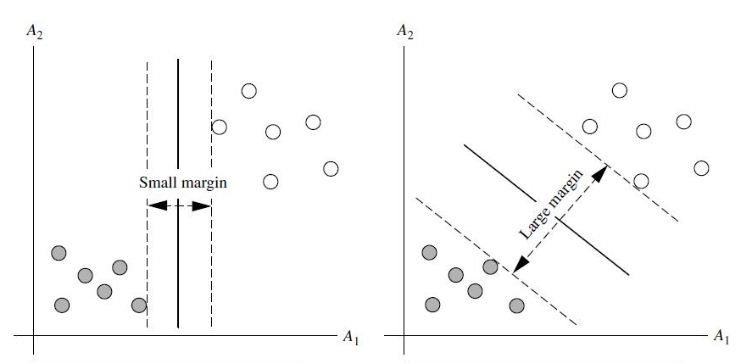
\includegraphics[width=.8\textwidth]{./Pictures/gesture/svm2.jpg}
        }
   }
   \caption{SVM With Possible Separating hyperplanes \cite{classifications}\label{fig:svm2} }   
\end{dBox}   
\end{figure*}

Getting to an informal definition of margin, we can say that the shortest distance from a hyperplane to one side of its margin is equal to the shortest distance from the hyperplane to the other side of its margin, where the "sides" of the margin are parallel to the hyperplane. When dealing with the MMH, this distance is, in fact, the shortest distance from the MMH to the closest training tuple of either class. A separating hyperplane can be written as $W.X+b = 0$  Where W is a weight vector, namely, W =${  w_1,w_2,...,w_n }$; n is the number of attributes; and b is a scalar, often referred to as a bias. To aid in visualization, let's consider two input attributes, A1 and A2, as in Figure \ref{fig:svm2} (b). Training tuples are 2-D (e.g., X = (x1, x2)), where x1 and x2 are the values of attributes A1 and A2, respectively, for X. If we think of b as an additional weight, w0, we can rewrite the previous equation as $w_{0} + w_{1} x_{1}+w_{2} x_{2}=0$ \bigskip

Thus, any point that lies above the separating hyperplane satisfies

\begin{dBox}
\begin{equation}
w_0 + w_1 x_1 + w_2  x_2 > 0 
\end{equation}
\end{dBox}

Similarly, any point that lies below the separating hyperplane satisfies

\begin{dBox}
\begin{equation}
w_0 + w_1 x_1 + w_2  x_2 < 0 
\end{equation}
\end{dBox}

The weights can be adjusted so that the hyperplanes defining the "sides" of the margin can be written as

\begin{dBox}
\begin{equation}
H_1: w_0 + w_1 x_1 + w_2 x_2 >= 1    $ for $  y_i = +1,
\end{equation}
\begin{equation}
H_2: w_0 + w_1 x_1 + w_2 x_2 =< -1    $ for $ y_i = -1
\end{equation}
\end{dBox}

That is, any tuple that falls on or above H1 belongs to class +1, and any tuple that falls on or below H2 belongs to class -1. Combining the two inequalities:

\begin{dBox}
\begin{equation}
y_{i}(w_0 + w_1 x_1 + w_2 x_2) >= 1 $ for all i$. 
\end{equation}
\end{dBox}
\bigskip
Any training tuples that fall on hyperplanes H1 or H2 (i.e., the "sides" defining the margin) satisfy the previous equation and are called support vectors. That is, they are equally close to the (separating) MMH. In \ref{fig:svm3}, the support vectors are shown encircled with a thicker border. Essentially, the support vectors are the most difficult tuples to classify and give the most information regarding classification.\bigskip
\bigskip
\begin{figure*}[h]
\begin{dBox}
\centering
  \mbox{
      \subfigure[]{
            \label{fig:svm_3}
            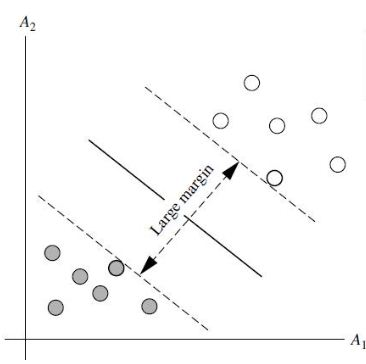
\includegraphics[width=.8\textwidth]{./Pictures/gesture/svm3.jpg}
        }
   }
   \caption{Higlight Support Vectors \cite{classifications}\label{fig:svm3} }   
\end{dBox}   
\end{figure*}

From this, we can obtain a formula for the size of the maximal margin. The distance from the separating hyperplane to any point on H1 is $1/|(|W|)|$, where $|(|W|)|$ is the Euclidean norm of W, that is, $\sqrt{W . W2}$. By definition, this is equal to the distance from any point on H2 to the separating hyperplane. Therefore, the maximal margin is $2/|(|W|)|$. Using some "fancy math tricks," we can rewrite the last equation so that it becomes what is known as a constrained (convex) quadratic optimization problem. Note that the tricks involve rewriting the last equation using a Lagrangian formulation and then solving for the solution using Karush-Kuhn-Tucker (KKT) conditions. If the data are small (say, less than 2000 training tuples), any optimization software package for solving constrained convex quadratic problems can then be used to find the support vectors and MMH. For larger data, special and more efficient algorithms for training SVMs can be used instead. Once we've found the support vectors and MMH (note that the support vectors define the MMH!), we have a trained support vector machine. The MMH is a linear class boundary, and so the corresponding SVM can be used to classify linearly separable data. We refer to such a trained SVM as a linear SVM.\bigskip

Based on the Lagrangian formulation mentioned before, the MMH can be rewritten as the decision boundary;

\begin{dBox}
\begin{equation}
d(X^{T}) = \sum_{i=1}^{l}{y_i \alpha_i X_i X^T} + b_0
\end{equation}
\end{dBox}

Where $y_i$  is the class label of support vector $X_i$ , $X^T$ is a test tuple; $\alpha_i$ and $b_0$ are numeric parameters that were determined automatically by the optimization or SVM algorithm noted before; and l is the number of support vectors. $\alpha_i$ are Lagrangian multipliers. For linearly separable data, the support vectors are a subset of the actual training tuples (although there will be a slight twist regarding this when dealing with non linearly separable data, as we shall see in the following).\bigskip

Given a test tuple, $X^T$, we plug it into last equation and then check to see the sign of the result. This tells us on which side of the hyperplane the test tuple falls. If the sign is positive, then $X^T$  falls on or above the MMH, and so the SVM predicts that $X^T$  belongs to class +1 (representing buys computer = yes, in our case). If the sign is negative, then $X^T$  falls on or below the MMH and the class prediction is -1 (representing buys computer = no). Notice that the Lagrangian formulation of our problem from the last equation contains a dot product between support vector $X_i$ and test tuple $X^T$. This will prove very useful for finding the MMH and support vectors for the case when the given data are non linearly separable, as described further in the next section. Before we move on to the nonlinear case, there are two more important things to note. The complexity of the learned classifier is characterized by the number of support vectors rather than the dimensionality of the data. Hence, SVMs tend to be less prone to overfitting than some other methods. The support vectors are the essential or critical training tuples-they lie closest to the decision boundary (MMH). If all other training tuples were removed and training were repeated, the same separating hyperplane would be found. Furthermore, the number of support vectors found can be used to compute an (upper) bound on the expected error rate of the SVM classifier, which is independent of the data dimensionality. An SVM with a small number of support vectors can have good generalization, even when the dimensionality of the data is high.

\subsubsection{Linear In-separability Of The Data}
The approach described for linear SVMs can be extended to create nonlinear SVMs for the classification of linearly inseparable data (also called nonlinearly separable data, or nonlinear data for short). Such SVMs are capable of finding nonlinear decision boundaries (nonlinear hypersurfaces) in input space. We obtain a nonlinear SVM by extending the approach for linear SVMs as follows. There are two main steps. In the first step, we transform the original input data into a higher dimensional space using a nonlinear mapping. Several common nonlinear mappings can be used in this step, as we will further describe next. Once the data have been transformed into the new higher space, the second step searches for a linear separating hyperplane in the new space. We again end up with a quadratic optimization problem that can be solved using the linear SVM formulation. The maximal marginal hyperplane found in the new space corresponds to a nonlinear separating hypersurface in the original space.\bigskip
\begin{figure*}[h]
\begin{dBox}
\centering
  \mbox{
      \subfigure[]{
            \label{fig:svm_4}
            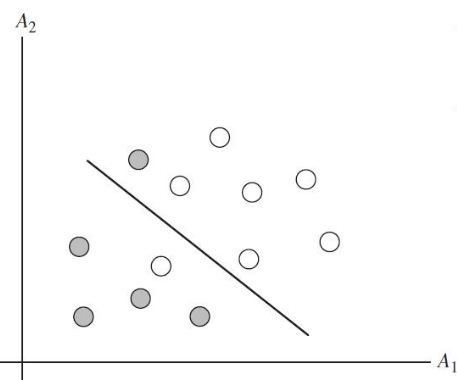
\includegraphics[width=.8\textwidth]{./Pictures/gesture/svm4.jpg}
        }
   }
   \caption{Linear In-separable Data \cite{classifications}\label{fig:svm4} }   
\end{dBox}   
\end{figure*}

However, there are some problems. First, how do we choose the nonlinear mapping to a higher dimensional space? Second, the computation involved will be costly. Referring to the last equation, for the classification of a test tuple, $X^T$. Given the test tuple, we have to compute its dot product with every one of the support vectors. In training, we have to compute a similar dot product several times in order to find the MMH. This is especially expensive. Hence, the dot product computation required is very heavy and costly.\bigskip

We can use another math trick. It so happens that in solving the quadratic optimization problem of the linear SVM (i.e., when searching for a linear SVM in the new higher dimensional space), the training tuples appear only in the form of dot products, $\phi{x_i }) $ .$\phi{x_j } $ , where $\phi{x_i }) $ is simply the nonlinear mapping function applied to transform the training tuples. Instead of computing the dot product on the transformed data tuples, it turns out that it is mathematically equivalent to instead apply a kernel function, $K(x_i,x_j )$  to the original input data. That is:
\begin{dBox}
\begin{equation}
K(x_i,x_j) = \phi{x_i} \phi{x_j}.
\end{equation}
\end{dBox}

In other words, everywhere that $\phi{x_i}$.$\phi{x_j}.$appears in the training algorithm, we can replace it with $K(x_i,x_j )$. In this way, all calculations are made in the original input space, which is of potentially much lower dimensionality! We can safely avoid the mapping-it turns out that we don't even have to know what the mapping is! We will talk more later about what kinds of functions can be used as kernel functions for this problem.

After applying this trick, we can then proceed to find a maximal separating hyperplane.\bigskip

Properties of the kinds of kernel functions that could be used to replace the dot product scenario just described have been studied. Three admissible kernel functions are:

\begin{itemize}
\item Polynomial kernel of degree $h: K(x_i,x_j )=(x_i.x_j+1)^h$.
\item Gaussian radial basis function kernel: $K(x_i,x_j )=e^-\frac{\|x_i- x_j \|^2}{2\sigma^2}$.
\item Sigmoid kernel: $K(x_i,x_j )=tanh(x_i.x_i-\delta)$.
\end{itemize}

Each of these results in a different nonlinear classifier in (the original) input space. Neural network aficionados will be interested to note that the resulting decision hyperplanes found for nonlinear SVMs are the same type as those found by other well-known neural network classifiers. For instance, an SVM with a Gaussian radial basis function (RBF) gives the same decision hyperplane as a type of neural network known as a radial basis function network. An SVM with a sigmoid kernel is equivalent to a simple two-layer neural network known as a multilayer perceptron (with no hidden layers). \bigskip

There are no golden rules for determining which admissible kernel will result in the most accurate SVM. In practice, the kernel chosen does not generally make a large difference in resulting accuracy. SVM training always finds a global solution, unlike neural networks, such as back propagation.
\bigskip

So far, we have described linear and nonlinear SVMs for binary (i.e., two-class) classification. SVM classifiers can be combined for the multiclass case.  A major research goal regarding SVMs is to improve the speed in training and testing so that SVMs may become a more feasible option for very large data sets (e.g., millions of support vectors). Other issues include determining the best kernel for a given data set and finding more efficient methods for the multiclass case.\bigskip

% SVM has the following results on our datasets. For Binary Representation Algorithm, it gives the best results according to the following results that describe the accuracy of ever static algorithm. \bigskip

% \begin{figure*}[h]
% \begin{dBox}
% \centering
%   \mbox{
%       \subfigure[]{
%             \label{fig:r_svm_bin}
%             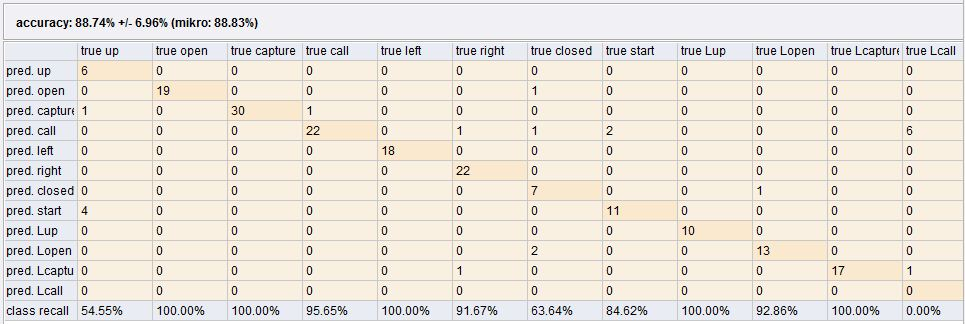
\includegraphics[width=.9\textwidth]{./Pictures/gesture/R_SVM_Binary.jpg}
%         }
%   }
%   \caption{Binary Based Approach Results Using x-validation with k=10\label{fig:r_svm_b} }   
% \end{dBox}   
% \end{figure*}

%\begin{figure*}[h]
%\begin{dBox}
%\centering
  %\mbox{
  %    \subfigure[]{
 %           \label{fig:r_svm_sift}
%            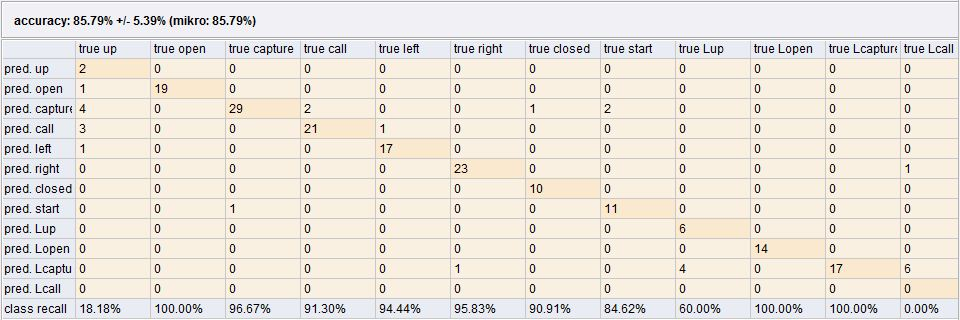
\includegraphics[width=.9\textwidth]{./Pictures/gesture%/R_SVM_SIFT.jpg}
   %     }
  % }
 %  \caption{SIFT and Bag Of Features Approach Results Using %x-validation with k=10\label{fig:r_svm_sift} }   
%\end{dBox}   
%\end{figure*}


% \begin{figure*}[h]
% \begin{dBox}
% \centering
%   \mbox{
%       \subfigure[]{
%             \label{fig:r_svm_fea}
%             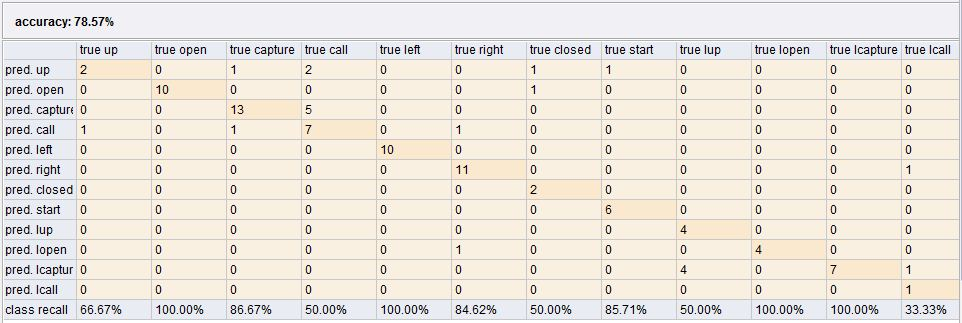
\includegraphics[width=.9\textwidth]{./Pictures/gesture/R_SVM_Feature.jpg}
%         }
%   }
%   \caption{Feature Based Approach Results Using x-validation with k=10\label{fig:r_svm_f} }   
% \end{dBox}   
% \end{figure*}


\subsection{KNN}\index{KNN}
The k-nearest-neighbor method \cite{classifications} was first described in the early 1950s. The method is labor intensive when given large training sets, and did not gain popularity until the 1960s when increased computing power became available. It has since been widely used in the area of pattern recognition. \bigskip

Nearest-neighbor classifiers are based on learning by analogy, that is, by comparing a given test tuple with training tuples that are similar to it. The training tuples are described by n attributes. Each tuple represents a point in an n-dimensional space. In this way, all the training tuples are stored in an n-dimensional pattern space.When given an unknown tuple, a k-nearest-neighbor classifier searches the pattern space for the k training tuples that are closest to the unknown tuple. These k training tuples are the k "nearest neighbors" of the unknown tuple.
\bigskip

"Closeness" is defined in terms of a distance metric, such as Euclidean distance. The
Euclidean distance between two points or tuples, say, $X1 =( x_{11}, x_{12},..., x_{1n})$ and $X2=(x_{21}, x_{22},..., x_{2n})$, is

\begin{dBox}
\begin{equation}
dist(x_1, x_2) = \sqrt{\sum_{i=1}^{n}(x_{1i}-x_{2i})^2}
\end{equation}
\end{dBox}


For k-nearest-neighbor classification, the unknown tuple is assigned the most common class among its k-nearest neighbors. When k = 1, the unknown tuple is assigned the class of the training tuple that is closest to it in pattern space. Nearest-neighbor classifiers can also be used for numeric prediction, that is, to return a real-valued prediction
for a given unknown tuple. In this case, the classifier returns the average value of the real-valued labels associated with the k-nearest neighbors of the unknown tuple.\bigskip

The previous discussion assumes that the attributes used
to describe the tuples are all numeric. For nominal attributes, a simple method is to compare the corresponding value of the attribute in tuple X1 with that in tuple X2. If
the two are identical (tuples X1 and X2 both have the color blue), then the difference between the two is taken as 0. If the two are different ( tuple X1 is blue but tuple X2 is red), then the difference is considered to be 1. Other methods may incorporate more sophisticated schemes for differential grading (where a larger difference score is assigned, say, for blue and white than for blue and black).\bigskip

"How can I determine a good value for k, the number of neighbors?" This can be determined experimentally. Starting with k = 1, we use a test set to estimate the error rate
of the classifier. This process can be repeated each time by incrementing k to allow for one more neighbor. The k value that gives the minimum error rate may be selected. In
general, the larger the number of training tuples, the larger the value of k will be (so that classification and numeric prediction decisions can be based on a larger portion of the stored tuples). As the number of training tuples approaches infinity and k = 1, the error rate can be no worse than twice the Bayes error rate (the latter being the theoretical minimum). If k also approaches infinity, the error rate approaches the Bayes error rate.\bigskip

Nearest-neighbor classifiers can be extremely slow when classifying test tuples. If D is a training database of |D| tuples and k = 1, then O(|D|) comparisons are required to
classify a given test tuple. By presorting and arranging the stored tuples into search trees, the number of comparisons can be reduced to O(log|D|). Parallel implementation can
reduce the running time to a constant, that is, O(1), which is independent of |D|. Other techniques to speed up classification time include the use of partial distance
calculations and editing the stored tuples. In the partial distance method, we compute the distance based on a subset of the n attributes. If this distance exceeds a threshold,
then further computation for the given stored tuple is halted, and the process moves on to the next stored tuple. The editing method removes training tuples that prove useless. This method is also referred to as pruning or condensing because it reduces the total
number of tuples stored.\bigskip
